\chapter{Multicast Communication}
Communication can be defined not only one-to-one, in fact there are other two possible cases:
\begin{itemize}
    \item \textbf{Broadcast \(\rightarrow\)} \textit{one-to-all communication:} a process send the ,estate to all the other processes
    \item \textbf{Multicast \(\rightarrow\)} \textit{one-to-many communication:} a process send the message to a specific group of processes
\end{itemize}
Multicast communication is very frequent and there are different motivations:
\begin{itemize}
    \item \textbf{Fault tolerance (server replication):} since the request is sent to a set of servers in parallel if one of them crash the other can reply to the request
    \item \textbf{Replication of data:}  data can be replicated in different servers
    \item \textbf{Performance:} the request can be executed by a group of servers in parallel, this approach improves the performance of the system
\end{itemize}
Multicast brings with it some issues for which it is needed to develop a solving strategy, like the fact that if  the sender sends a request to a group of servers, how does it has to deal with the answer? There can be different strategy, like:
\begin{itemize}
    \item No wait
    \item Wait only for some answer, but how many
    \item Wait for all the answer
\end{itemize}

\begin{figure}[!h]
    \centering
    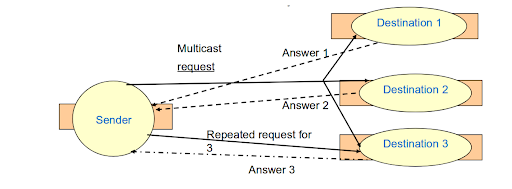
\includegraphics[width=.7\linewidth]{images/multicastCommunication/multicastcomm.png}
    \caption{Example of Multicast Communication}
\end{figure}


\section{Atomicity and Reliability Definitions}
Multicast communication can also provide two mainly features:
\begin{itemize}
    \item \textbf{Atomicity:} which guarantee that all the component inside the group will receive the message
    \item \textbf{Reliability:} which guaranteed the delivery:
        \begin{itemize}
            \item \textit{Validity:} messages are delivered
            \item \textit{Integrity:} messages that are delivered at most once are correct
            \item \textit{Agreement:} messages are delivered to all the destination processes
        \end{itemize}
\end{itemize}
An \textbf{unreliable multicast} communication system \underline{sends only once the message.}

\section{Ordering}
Another important issue from multicast protocol is \textbf{ordering}, messages are transmitted to a group in multicast and arrive to each component of the group according to the sending order. Taking this example:

\begin{figure}[!h]
    \centering
    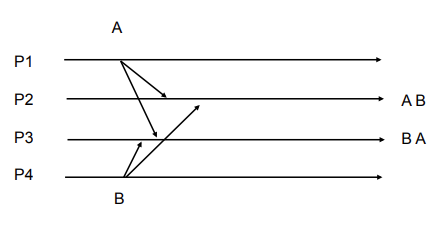
\includegraphics[width=.7\linewidth]{images/multicastCommunication/orderingProblemMulticast.PNG}
    \caption{Ordering Problem in Multicast}
\end{figure}

A and B are two events sent by two different senders and A is sent before B. Ordering problem consists of developing a \ul{strategy that ensures that receivers receive the two messages with the same order.} \textbf{Single Atomic Multicast} keeps the FCFS order of the messages, so when there is only one sender the order is guaranteed. Instead considering if there are multiple senders this strategy does not ensure the order, so we have to considered three solving methods:
\begin{itemize}
    \item \textbf{FIFO ordering:}  where it preserves the order from the perspective of a sender process. (the order is the same of the sender process)
    \item \textbf{Casual ordering:} where it considers a \underline{logical ordering}, called also \underline{casual}, and the message is delivered considering that constraint, so if an event A precedes an event B then the messages are delivered according to that order
    \item \textbf{Totally ordered multicast:} if it is atomic, it delivers the message to each member of the group in the same order
\end{itemize}

\section{Implementations}
Multicast can be supported by different types of implementations of the two primitives: \textit{send}  and \textit{receive}. The way the two are implemented define the multicast system. Next we see a basic implementation of send primitive, \textbf{not reliable and atomic.}

\begin{figure}[!h]
    \centering
    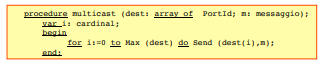
\includegraphics[width=.7\linewidth]{images/multicastCommunication/multicastimplementation.png}
    \caption{Example of Multicast Implementation}
\end{figure}

For a reliable multicast is necessary to check the following assets:
\begin{itemize}
    \item Possible message loss
    \item Crashing of sender
    \item Wait the answer
    \item Possible retransmission in case of time out
\end{itemize}
The implementation of the fault management system have to take into account the occurrence of faults like:
\begin{itemize}
    \item Message omission
    \item Sender crash
\end{itemize}
A possible solution is to use a \textbf{monitor} with the following rules:
\begin{itemize}
    \item Check of current transmission
    \item Manage possible retransmission
    \item Remove crashed processes: if a process is waiting for an \textbf{ack}  but the server crashed it will wait for ever
    \item Notifies the group’s components when a process is added or executed
\end{itemize}

\section{Reliability and Atomicity in practise}
Atomicity and reliability bring with them a non indifferent cost since:
\begin{itemize}
    \item \textbf{Sender} sends the message to the group and waits for the ack from all the components inside the group
    \item If all the \textbf{ack} arrive it is ok, otherwise if they do not arrive within a timeout it is necessary to re-transmit the message
\end{itemize}
Another problem for \textbf{atomicity} regards the management of \textbf{sender fault.} 
In this case to preserve atomicity every destination process sends an ack and waits for confirm, the sender once the multicast is completed sends back to confirm to everyone, but this solution is \textbf{not so efficient}, and so we can consider \textbf{Hold-back queue} as alternative.
With \textbf{Hold-back queue} the destination keeps the message suspended before delivery, up to the arrival of the confirm. In order to guarantee the ordering and atomicity the messages are numbered and every message is delayed until the previous ones arrive.

\begin{figure}[!h]
    \centering
    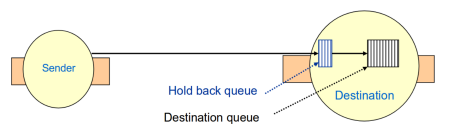
\includegraphics[width=.7\linewidth]{images/multicastCommunication/reliabilityatomicity.png}
    \caption{Hold'back Queue}
\end{figure}

Another solution consists to the usage of \textbf{negative ack:}
\begin{itemize}
    \item The messages are numbered according to the order from the server
    \item The destination process sends a \textbf{NACK} if the message number of the arrival \underline{is not in the order of the sequence}
    \item The destination process does not send the \textbf{ACK}
    \item The sender has a \textbf{copy} (history) of the \textbf{sent messages}
\end{itemize}
The sender has a copy (history) of the sent messages
But using only ack is difficult to understand when it’s time to clear the history, so occasionally destination processes send positive ack with number of received messages using piggybacking technique.


\section{Atomic and totally order multicast}
In order to guarantee atomicity and totally order each process is associated with a \textbf{unique totally ordered identifier.}
A message is \textbf{stable} in the destination if other messages with smaller identifiers cannot arrive.

This solution is easy to implement if sender and receivers agree with \textbf{a shared identifier sequence} used to assign identifiers to the messages. In order to decide this sequence some solutions are proposed:
\begin{itemize}
    \item Using a timestamp from physical or logical clock
    \item Using a sequencer process
    \item Using a protocol among the group processes to generate an identifier
\end{itemize}
Regarding the implementation it can defined:
\begin{itemize}
    \item \textbf{Centraized:} unique manager that makes the ordering. But the drawback is that it can become a bottleneck since all the request should pass from him
    \item \textbf{Distributed:} coordination of the receivers that makes an agreement on the ordering
\end{itemize}

\begin{figure}[!h]
    \centering
    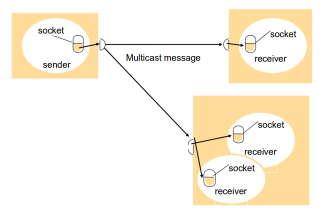
\includegraphics[width=.7\linewidth]{images/multicastCommunication/totalyordered.png}
    \caption{Atomic and Totally ordered Multicast}
\end{figure}